% IEEE Open Journal of Intelligent Transportation Systems
% metroLM: A Taxonomy-Driven Family of Metro Language Models
% with TAKTKRONE-I for Operations Control Center Decision Support

\documentclass[journal]{IEEEtran}

\usepackage{cite}
\usepackage{amsmath,amssymb,amsfonts}
\usepackage{algorithmic}
\usepackage{graphicx}
\usepackage{textcomp}
\usepackage{xcolor}
\usepackage{booktabs}
\usepackage{multirow}
\usepackage{array}
\usepackage{url}
\usepackage{hyperref}

\hypersetup{
    colorlinks=true,
    linkcolor=black,
    citecolor=black,
    urlcolor=blue
}

\begin{document}

\title{metroLM: A Taxonomy-Driven Family of Metro Language Models with TAKTKRONE-I for Operations Control Center Decision Support}

\author{Gustav~Olaf~Yunus~Laitinen-Fredriksson~Lundstr\"{o}m-Imanov
\thanks{G. O. Y. Laitinen-Fredriksson Lundstr\"{o}m-Imanov is an independent researcher. Contact: dev@taktkrone.ai. Project website: https://taktkrone.ai. Code and data: https://github.com/olaflaitinen/taktkrone-i.}}

\markboth{IEEE Open Journal of Intelligent Transportation Systems, Vol.~X, No.~X, 2026}
{Laitinen-Fredriksson Lundstr\"{o}m-Imanov: metroLM and TAKTKRONE-I for Metro OCC Decision Support}

\maketitle

\begin{abstract}
Metro operations control centers face increasing complexity in managing disruptions, regulating headways, coordinating turnbacks, and planning service recovery under real-time constraints. Existing decision support tools remain fragmented, lacking the integrated reasoning capabilities required for holistic incident response. This paper introduces metroLM, a taxonomy-driven family of specialized language models for metro transit systems, and presents TAKTKRONE-I as the flagship instantiation of occLM, the Operations Control Center subfamily. TAKTKRONE-I integrates public transit data standards including GTFS Schedule and GTFS Realtime with synthetic OCC supervision traces to enable disruption summarization, delay diagnosis, action recommendation ranking, and uncertainty-aware operational guidance. The model architecture incorporates retrieval-augmented grounding, structured output contracts, and explicit human review boundaries to ensure that all recommendations require dispatcher validation before operational action. We evaluate TAKTKRONE-I on a simulation-backed benchmark spanning eight disruption severity levels and six task families, comparing against generic instruction-tuned baselines, retrieval-augmented alternatives, and rule-based heuristics. Results demonstrate that taxonomy-grounded specialization combined with domain-specific supervision yields improvements in summarization quality (ROUGE-L 0.678 versus 0.412 for generic baselines), recommendation ranking (nDCG@5 0.812 versus 0.534), and calibration error reduction (ECE 0.067 versus 0.183). The system explicitly labels uncertainty, refuses unsafe requests at 94.3\% accuracy, and maintains topology consistency at 96.7\%. All results are derived from public data sources and synthetic benchmarks; no claims of operational deployment or safety certification are made.
\end{abstract}

\begin{IEEEkeywords}
Metro operations control, intelligent transportation systems, large language models, rail disruption management, GTFS Realtime, decision support, urban rail transit
\end{IEEEkeywords}

\section{Introduction}
\label{sec:introduction}

\IEEEPARstart{M}{etro} operations control centers serve as the cognitive hub of urban rail transit systems, coordinating real-time responses to service disruptions, passenger flow anomalies, and infrastructure incidents. Controllers must synthesize information from multiple sources, including train tracking systems, passenger information displays, communication-based train control telemetry, and service alert feeds, to make time-critical decisions about headway regulation, dwell control, short-turn maneuvers, and line recovery strategies \cite{ceder2016public, hansen2014railway}. The complexity of these decisions has grown substantially as metro networks expand, ridership increases, and service frequency targets become more aggressive.

Despite advances in railway operations research \cite{dariano2007conflict, goverde2010delay, corman2010tabu}, existing decision support tools for metro OCC remain fragmented. Dispatchers typically work with separate interfaces for train tracking, passenger counting, incident logging, and service planning, requiring mental integration across systems that were not designed for unified reasoning. Rule-based expert systems provide deterministic guidance for common scenarios but struggle with novel combinations of failures or cascading delays \cite{botte2018dispatching}. Statistical models can predict delay propagation \cite{buchel2020empirical, dekker2022modelling} but do not generate actionable natural language recommendations that explain reasoning or quantify uncertainty.

The emergence of large language models (LLMs) offers a potential pathway toward more integrated decision support \cite{brown2020language, ouyang2022training}. However, applying general-purpose LLMs to safety-relevant transportation domains presents significant challenges. Generic models lack grounding in transit data standards, network topology constraints, and operational feasibility requirements \cite{wandelt2024large, hassija2025role}. They may generate plausible-sounding but operationally invalid recommendations, hallucinate station names or line configurations, or fail to recognize when a proposed action violates safety boundaries \cite{ji2023survey}.

This paper addresses these challenges through two primary contributions. First, we introduce metroLM, a taxonomy-driven family of specialized language models for metro transit systems. The metroLM taxonomy organizes domain specialization across 29 categories spanning four tiers, from foundational transit knowledge through operational reasoning to cross-domain integration. This structured approach enables targeted model development rather than attempting to solve all metro AI problems with a single architecture.

Second, we present TAKTKRONE-I as the flagship instantiation of occLM, the Operations Control Center subfamily within metroLM. TAKTKRONE-I is designed specifically for disruption-time decision support, combining retrieval-augmented generation over public transit data with synthetic OCC supervision to enable delay diagnosis, service recovery planning, and uncertainty-aware recommendation generation. The system architecture enforces explicit human review boundaries and refuses to provide guidance that would bypass dispatcher oversight.

Our evaluation employs a simulation-backed benchmark constructed from public GTFS feeds and synthetic OCC dialogue traces. We compare TAKTKRONE-I against generic instruction-tuned baselines, retrieval-augmented alternatives, and traditional rule-based heuristics across six task families and eight disruption severity levels. Results demonstrate meaningful improvements in summarization quality, recommendation ranking, and calibration while maintaining high rates of topology consistency and unsafe request refusal.

The research questions guiding this work are:

\begin{enumerate}
    \item Can a taxonomy-driven approach to LLM specialization improve domain fidelity for metro OCC reasoning compared to generic fine-tuning?
    \item Does synthetic OCC supervision, grounded in public transit data standards, yield actionable guidance that maintains operational validity constraints?
    \item How should uncertainty-aware output contracts be designed to support human-in-the-loop decision making rather than autonomous action?
\end{enumerate}

The primary contributions of this paper are:

\begin{itemize}
    \item A structured metroLM taxonomy for metro-domain language model specialization, organizing 29 categories across four tiers with explicit cross-domain convergence.
    \item A technical architecture for TAKTKRONE-I as the occLM implementation, integrating GTFS grounding, retrieval augmentation, and uncertainty-aware structured outputs.
    \item A public-data-plus-synthetic supervision pipeline demonstrating how to construct OCC training data without access to proprietary dispatcher telemetry.
    \item A simulation-backed evaluation framework covering disruption diagnosis, service recovery, and calibration quality with explicit comparison against multiple baselines.
\end{itemize}

The remainder of this paper is organized as follows. Section~\ref{sec:related} reviews related work on LLMs for transportation, railway operations research, and transit data standards. Section~\ref{sec:taxonomy} presents the metroLM taxonomy and positions occLM within it. Section~\ref{sec:architecture} describes the TAKTKRONE-I system architecture. Section~\ref{sec:data} details the data sources, supervision approach, and benchmark design. Section~\ref{sec:results} presents experimental results and ablations. Section~\ref{sec:safety} discusses safety considerations, limitations, and threats to validity. Section~\ref{sec:conclusion} concludes with future directions.

\section{Related Work}
\label{sec:related}

This section reviews four clusters of related work: large language models and foundation models, LLMs for intelligent transportation systems, railway delay management and dispatching, and metro signalling with real-time transit data standards.

\subsection{Large Language Models and Foundation Models}

The transformer architecture \cite{vaswani2017attention} enabled a paradigm shift in natural language processing, leading to pretrained models such as BERT \cite{devlin2019bert} and T5 \cite{raffel2020exploring} that established transfer learning as the dominant approach. Scaling studies demonstrated emergent capabilities in models trained on massive corpora \cite{brown2020language}, while instruction tuning and reinforcement learning from human feedback improved alignment with user intent \cite{ouyang2022training}. Chain-of-thought prompting revealed that explicit reasoning steps improve performance on complex tasks \cite{wei2022chain}.

Efficient adaptation methods such as LoRA \cite{hu2022lora} and QLoRA \cite{dettmers2023qlora} enable domain specialization without full model retraining, making it feasible to develop targeted models for specific application domains. Open foundation models including LLaMA \cite{touvron2023llama, touvron2023llama2} provide accessible bases for specialized fine-tuning. However, foundation model risks including hallucination \cite{ji2023survey}, calibration failures \cite{guo2017calibration}, and ethical concerns \cite{bender2021dangers, weidinger2022ethical} require careful mitigation in safety-relevant domains.

Retrieval-augmented generation \cite{lewis2020retrieval} addresses some hallucination concerns by grounding model outputs in retrieved evidence, though retrieval quality directly impacts generation quality. Model cards \cite{mitchell2019model} and datasheets \cite{gebru2021datasheets} establish documentation standards for responsible model development.

\subsection{LLMs for Intelligent Transportation Systems}

Application of LLMs to transportation domains has accelerated recently. Wandelt et al. \cite{wandelt2024large} survey LLM applications across traffic prediction, autonomous vehicles, and public transit, identifying opportunities for natural language interfaces to transportation data. Gan et al. \cite{gan2024large} review large models for intelligent transportation and autonomous vehicles, emphasizing multimodal integration challenges. Hassija et al. \cite{hassija2025role} examine LLM roles in enhancing intelligent transportation systems, noting gaps in domain-specific evaluation.

TransitGPT \cite{devunuri2025transitgpt} demonstrates LLM-assisted knowledge generation for public transportation, using GTFS data to answer passenger queries about routes and schedules. This passenger-facing application differs from our OCC-facing focus but validates the utility of GTFS grounding for transit LLMs. Several studies explore LLMs for traffic forecasting and incident detection, though these typically treat the LLM as a feature extractor rather than a reasoning engine.

A notable gap exists at the intersection of LLMs and metro operations control. Existing transit LLM work focuses primarily on passenger information, travel planning, or traffic prediction rather than dispatcher decision support. Our work addresses this gap by targeting OCC-specific tasks including disruption diagnosis, headway regulation reasoning, and service recovery planning.

\subsection{Railway Delay Management and Dispatching}

Railway operations research has developed extensive theory for delay management, train rescheduling, and conflict resolution. D'Ariano et al. \cite{dariano2007conflict} present algorithms for real-time timetable perturbation resolution, optimizing train speeds and routing to minimize delay propagation. Goverde \cite{goverde2010delay} introduces delay propagation algorithms for large-scale networks based on max-plus algebra. Corman et al. \cite{corman2010tabu} apply tabu search to train rerouting during disruptions.

K\"onig \cite{konig2020review} provides a comprehensive review of railway delay management, categorizing approaches by objective function, solution method, and real-time applicability. B\"uchel et al. \cite{buchel2020empirical} empirically analyze delay propagation dynamics during the large-scale Rastatt disruption, revealing complex cascade patterns. Dekker et al. \cite{dekker2022modelling, dekker2021geographic} model delay propagation as diffusion-like spreading and characterize geographic patterns in railway delay.

Recent work by Liu et al. \cite{liu2023prediction, liu2023automatic} explores delay propagation prediction using causal text information extracted from incident reports, representing an early intersection of NLP and railway operations. However, these approaches focus on prediction rather than decision support and do not generate natural language recommendations.

Passenger flow control emerges as an increasingly important dimension of metro operations. Yatziv and Haddad \cite{yatziv2025realtime} present real-time train regulation with passenger flow control, integrating demand management with supply-side interventions. Li et al. \cite{li2025formulation} formulate train-passenger-station interactive simulation for influx control evaluation. Xing et al. \cite{xing2026joint} apply multi-agent reinforcement learning to joint optimization of passenger flow control and train skip-stopping. These optimization approaches could potentially be integrated with LLM-based reasoning in future work.

\subsection{Metro Signalling and Real-Time Transit Data Standards}

Communication-based train control (CBTC) systems provide the technical foundation for modern metro operations, enabling moving block signalling and automatic train operation \cite{li2016fuzzy, huang2021research}. Chang et al. \cite{chang2022architecture} examine software-defined architectures for next-generation train control with reliability considerations. Su et al. \cite{su2023simulation} present simulation methods for calculating passenger flow distribution during service interruptions.

The General Transit Feed Specification (GTFS) has become the dominant standard for public transit data exchange. GTFS Schedule \cite{gtfs_schedule} defines static timetable and network topology information, while GTFS Realtime \cite{gtfs_realtime} extends this with trip updates, vehicle positions, and service alerts. MobilityData \cite{mobilitydata} maintains the specification and publishes best practices \cite{gtfs_best_practices}.

GTFS Realtime provides three primary feed types relevant to OCC decision support. Trip updates \cite{gtfs_trip_updates} contain arrival and departure predictions for individual trips, enabling delay quantification. Vehicle positions \cite{gtfs_vehicle_positions} report real-time locations, supporting headway calculation and gap detection. Service alerts \cite{gtfs_service_alerts} communicate disruption information in structured form with affected entities and time ranges.

A critical limitation of public GTFS feeds is the absence of dispatcher rationale. Feeds report what is happening (delays, positions, alerts) but not why dispatchers made particular decisions or what alternatives were considered. This motivates our use of synthetic OCC supervision to fill the reasoning gap.

\section{metroLM Taxonomy and Position of occLM}
\label{sec:taxonomy}

This section presents the metroLM taxonomy as a structured framework for metro-domain language model specialization and positions occLM as the Operations Control Center subfamily.

\subsection{Taxonomy Design Principles}

The metroLM taxonomy is designed around three principles. First, \textit{operational grounding}: categories must correspond to distinct operational roles within metro systems rather than abstract technical capabilities. Second, \textit{data modality alignment}: categories should align with available data sources to enable targeted training data construction. Third, \textit{composability}: categories should support integration through a cross-domain convergence layer rather than requiring monolithic models.

\subsection{Four-Tier Organization}

The taxonomy organizes 29 categories across four tiers:

\textbf{Tier 1: Foundational Transit Knowledge} encompasses basic transit concepts, network topology representation, timetable semantics, and passenger flow fundamentals. Models at this tier can answer factual questions about routes, stations, and schedules but lack operational reasoning capabilities.

\textbf{Tier 2: Real-Time Situational Awareness} covers vehicle tracking interpretation, delay quantification, service alert parsing, and headway analysis. Models at this tier process GTFS Realtime feeds and related telemetry to produce structured situational summaries.

\textbf{Tier 3: Operational Reasoning} includes disruption diagnosis, recovery planning, resource allocation, and intervention prioritization. This tier contains occLM, the Operations Control Center subfamily that TAKTKRONE-I instantiates.

\textbf{Tier 4: Cross-Domain Convergence} enables integration across tiers, combining situational awareness with operational reasoning and foundational knowledge to produce coherent multi-step recommendations.

\subsection{occLM and TAKTKRONE-I}

The occLM subfamily targets Operations Control Center decision support with nine primary capabilities: headway regulation support, dwell control reasoning, turnback management support, dispatch conflict resolution, line recovery planning, disruption summarization, delay diagnosis, structured extraction from service alerts, and uncertainty-aware operational recommendation.

TAKTKRONE-I is the first instantiated model within occLM, focusing on text-based reasoning over GTFS-grounded scenarios. The name reflects Nordic origins (Swedish/Danish tak for acknowledgment, krone for crown/top) combined with the designation I for the inaugural version. Future occLM models may incorporate multimodal inputs (platform camera feeds, audio communications) or specialized architectures for specific metro operators.

Table~\ref{tab:taxonomy} summarizes the metroLM taxonomy with occLM placement.

\begin{table*}[t]
\centering
\caption{metroLM Taxonomy Summary with occLM Placement}
\label{tab:taxonomy}
\begin{tabular}{@{}lllll@{}}
\toprule
\textbf{Tier} & \textbf{Category Family} & \textbf{Example Model} & \textbf{Primary Operational Role} & \textbf{Data Modalities} \\
\midrule
1 & Transit Knowledge & baseMetro & Factual Q\&A about routes and schedules & GTFS Schedule, documentation \\
1 & Topology Reasoning & topoLM & Network structure and connectivity analysis & Graph representations, GTFS stops \\
2 & Realtime Awareness & rtLM & Situational summary from live feeds & GTFS Realtime, vehicle positions \\
2 & Alert Processing & alertLM & Structured extraction from service alerts & Service alerts, incident reports \\
3 & Operations Control & \textbf{occLM (TAKTKRONE-I)} & \textbf{OCC decision support} & \textbf{All above + synthetic OCC traces} \\
3 & Recovery Planning & recoveryLM & Service restoration optimization & Timetables, resource constraints \\
4 & Convergence & metroLM-full & Multi-tier integrated reasoning & All modalities \\
\bottomrule
\end{tabular}
\end{table*}

\section{TAKTKRONE-I System Architecture}
\label{sec:architecture}

This section describes the technical architecture of TAKTKRONE-I, including input processing, reasoning modules, retrieval grounding, output contracts, and safety boundaries.

\subsection{Input Layers}

TAKTKRONE-I processes five input layers:

\textbf{GTFS Static}: Network topology including stations, lines, routes, and scheduled stop times. This provides the foundational knowledge of what services should be operating.

\textbf{GTFS Realtime}: Trip updates with arrival/departure predictions, vehicle positions for location tracking, and service alerts for official disruption communication.

\textbf{Topology Metadata}: Graph structure encoding station connectivity, transfer points, terminal stations suitable for turnbacks, and depot locations.

\textbf{Service Alerts}: Structured disruption information including affected routes, time ranges, cause categories, and passenger impact descriptions.

\textbf{Synthetic Scenario Memory}: Retrieved examples of similar past scenarios with dispatcher actions and outcomes, enabling few-shot reasoning over historical patterns.

\subsection{Reasoning Modules}

The architecture includes four primary reasoning modules:

\textbf{Disruption Summarization}: Synthesizes multi-source inputs into concise operational summaries, highlighting the most critical information for dispatcher attention.

\textbf{Delay Diagnosis}: Analyzes delay patterns to identify root causes, distinguishing primary disruptions from cascading effects and estimating propagation trajectories.

\textbf{Action Ranking}: Generates candidate recovery actions and ranks them by estimated effectiveness, feasibility, and passenger impact, with explicit uncertainty quantification.

\textbf{Uncertainty Estimation}: Labels all outputs with confidence levels and identifies information gaps that prevent definitive recommendations.

\subsection{Retrieval Grounding Layer}

Following retrieval-augmented generation principles \cite{lewis2020retrieval}, TAKTKRONE-I grounds reasoning in retrieved evidence from a vector store of operational knowledge. The retrieval corpus includes:

\begin{itemize}
    \item GTFS-derived reference material on routes and schedules
    \item Service alert history with resolution outcomes
    \item Synthetic OCC dialogue examples
    \item Operational procedure documentation
\end{itemize}

Retrieved passages are incorporated into the model context with explicit source attribution, enabling the model to cite evidence for its recommendations.

\subsection{Structured Output Contract}

TAKTKRONE-I produces outputs conforming to a structured contract:

\begin{verbatim}
{
  "summary": <string>,
  "diagnosis": {
    "primary_cause": <string>,
    "confidence": <float 0-1>,
    "contributing_factors": [<string>]
  },
  "recommendations": [
    {
      "action": <string>,
      "priority": <int 1-5>,
      "confidence": <float 0-1>,
      "rationale": <string>,
      "risks": [<string>]
    }
  ],
  "uncertainty_flags": [<string>],
  "review_required": <boolean>,
  "refused": <boolean>,
  "refusal_reason": <string | null>
}
\end{verbatim}

The \texttt{review\_required} field is always true for action recommendations, enforcing human validation. The \texttt{refused} field activates when requests would bypass safety boundaries.

\subsection{Human Review Boundary}

TAKTKRONE-I is explicitly designed as a decision support system, not an autonomous controller. The architecture enforces several boundaries:

\begin{enumerate}
    \item All action recommendations require dispatcher confirmation
    \item The model never issues direct commands to train control systems
    \item Safety-critical decisions (e.g., track intrusion response) trigger immediate escalation rather than recommendation
    \item Uncertainty above threshold triggers explicit ``insufficient information'' responses rather than forced recommendations
\end{enumerate}

\subsection{Safety Guardrails}

Input guardrails filter requests that would require the model to:
\begin{itemize}
    \item Generate commands for direct train control
    \item Bypass established safety protocols
    \item Provide guidance beyond its training domain
    \item Speculate about equipment conditions without telemetry evidence
\end{itemize}

Output guardrails verify that generated recommendations:
\begin{itemize}
    \item Reference only valid stations and lines from the topology
    \item Do not propose physically impossible movements
    \item Include appropriate uncertainty qualification
    \item Maintain temporal consistency with the scenario timeline
\end{itemize}

\section{Data, Supervision, and Benchmark Design}
\label{sec:data}

This section describes the data sources, supervision approach, and evaluation benchmark for TAKTKRONE-I.

\subsection{Data Sources}

Table~\ref{tab:data_composition} summarizes the data composition.

\begin{table*}[t]
\centering
\caption{TAKTKRONE-I Data and Supervision Composition}
\label{tab:data_composition}
\begin{tabular}{@{}lllll@{}}
\toprule
\textbf{Source Layer} & \textbf{Example Data} & \textbf{Role in Training} & \textbf{Role in Evaluation} & \textbf{Public/Synthetic} \\
\midrule
GTFS Schedule & Routes, stops, stop\_times & Topology grounding & Consistency validation & Public \\
GTFS Realtime & Trip updates, vehicle positions & Scenario construction & Test scenario inputs & Public \\
Service Alerts & Disruption announcements & Alert parsing training & Structured extraction eval & Public \\
Synthetic OCC Traces & Dispatcher dialogue samples & Primary supervision & Benchmark test cases & Synthetic \\
Operational Procedures & Standard operating procedures & Retrieval corpus & Factual consistency check & Public/Constructed \\
\bottomrule
\end{tabular}
\end{table*}

\textbf{Public GTFS Data}: We collected GTFS Schedule and GTFS Realtime feeds from five transit agencies (MTA NYCT, MBTA, WMATA, BART, TfL) over a six-month period, yielding topology definitions for analysis and real delay patterns for scenario construction.

\textbf{Synthetic OCC Supervision}: Because public feeds lack dispatcher reasoning, we constructed synthetic OCC dialogue traces through a structured generation process:

\begin{enumerate}
    \item Extract disruption scenarios from historical GTFS Realtime anomalies
    \item Define plausible dispatcher queries for each scenario type
    \item Generate response templates following operational procedure guidelines
    \item Apply variation through paraphrasing and scenario modification
    \item Validate for topology consistency and operational feasibility
\end{enumerate}

This process yielded 5,247 OCC dialogue samples spanning multiple task families.

\subsection{Task Families}

We define six task families for OCC decision support:

\textbf{State to Summary}: Given network state from GTFS Realtime, produce a concise dispatcher briefing highlighting anomalies and priorities.

\textbf{State to Action Recommendation}: Given state plus specific query, recommend ranked actions with rationale and uncertainty quantification.

\textbf{Advisory to Structured Event}: Parse service alert text into structured event records with affected entities, time ranges, and cause categories.

\textbf{Timeline to After-Action Review}: Given incident timeline, produce structured post-incident analysis identifying decision points and outcomes.

\textbf{Incomplete Telemetry to Uncertainty-Aware Answer}: Given partial or conflicting information, produce appropriately hedged responses that acknowledge information gaps.

\textbf{Unsafe Request to Refusal}: Identify requests that would bypass safety boundaries and produce appropriate refusal responses.

\subsection{Benchmark Scenarios}

The evaluation benchmark includes eight severity levels:

\begin{enumerate}
    \item Normal operations (routine monitoring)
    \item Minor disturbance (single delayed train)
    \item Moderate disruption (multiple delays, potential cascading)
    \item Severe disruption (line segment suspended)
    \item Terminal failure (terminal station unavailable)
    \item Sparse telemetry (missing vehicle positions)
    \item Conflicting evidence (inconsistent data sources)
    \item No-action-needed (anomaly resolving naturally)
\end{enumerate}

\subsection{Evaluation Metrics}

We employ the following metrics:

\textbf{Summarization Quality}: ROUGE-1, ROUGE-2, ROUGE-L scores against reference summaries.

\textbf{Recommendation Ranking}: nDCG@5 and nDCG@10 for action ranking against expert orderings.

\textbf{Schema Validity}: Percentage of outputs conforming to the structured contract.

\textbf{Topology Consistency}: Percentage of outputs referencing only valid stations and feasible movements.

\textbf{Temporal Consistency}: Percentage of outputs with internally consistent timeline references.

\textbf{Calibration}: Expected Calibration Error (ECE) measuring alignment between stated confidence and actual correctness.

\textbf{Refusal Correctness}: Accuracy of refusing unsafe requests while accepting valid ones.

Table~\ref{tab:benchmark} summarizes the benchmark design.

\begin{table*}[t]
\centering
\caption{Benchmark Tasks, Metrics, and Baselines}
\label{tab:benchmark}
\begin{tabular}{@{}lllll@{}}
\toprule
\textbf{Task} & \textbf{Output Type} & \textbf{Primary Metric} & \textbf{Secondary Metric} & \textbf{Baselines} \\
\midrule
State to Summary & Text & ROUGE-L & BERTScore & Generic LLM, RAG-LLM \\
State to Recommendation & Structured JSON & nDCG@5 & Schema validity & Generic LLM, RAG-LLM, Rules \\
Advisory Extraction & Structured JSON & Macro F1 & Field accuracy & Generic LLM, Regex \\
After-Action Review & Text & ROUGE-L & Timeline accuracy & Generic LLM \\
Uncertainty Response & Structured JSON & Calibration (ECE) & Hedge accuracy & Generic LLM \\
Unsafe Request Refusal & Boolean + text & Refusal F1 & False positive rate & Generic LLM, Keyword filter \\
\bottomrule
\end{tabular}
\end{table*}

\section{Experimental Results}
\label{sec:results}

This section presents experimental results comparing TAKTKRONE-I against baselines and ablations. All results are derived from simulation-backed benchmarks using public data and synthetic supervision; no operational deployment evidence is claimed.

\subsection{Baselines}

We compare against four baselines:

\textbf{Generic LLM}: Llama 3.1 8B Instruct without domain-specific fine-tuning, using in-context examples from our benchmark.

\textbf{RAG-Generic}: Generic LLM augmented with retrieval over GTFS documentation and operational procedures, without OCC-specific training.

\textbf{Rules-Based}: Deterministic rule engine encoding common operational heuristics for delay response.

\textbf{TAKTKRONE-I w/o Retrieval}: Ablation removing the retrieval grounding layer.

\textbf{TAKTKRONE-I w/o Synth}: Ablation trained without synthetic OCC supervision, using only GTFS-derived data.

\textbf{TAKTKRONE-I w/o Uncertainty}: Ablation removing explicit uncertainty estimation from the output contract.

\subsection{Main Results}

Table~\ref{tab:results} presents main results across all methods.

\begin{table*}[t]
\centering
\caption{Main Results and Ablations (Simulation-Backed Benchmark)}
\label{tab:results}
\begin{tabular}{@{}lccccc@{}}
\toprule
\textbf{Method} & \textbf{ROUGE-L} & \textbf{nDCG@5} & \textbf{Schema (\%)}& \textbf{ECE ($\downarrow$)} & \textbf{Refusal Acc (\%)} \\
\midrule
Generic LLM & 0.412 & 0.534 & 67.3 & 0.183 & 71.2 \\
RAG-Generic & 0.487 & 0.612 & 72.8 & 0.156 & 74.8 \\
Rules-Based & 0.298 & 0.478 & 98.7 & -- & 89.4 \\
\midrule
TAKTKRONE-I w/o Retrieval & 0.589 & 0.723 & 94.2 & 0.098 & 88.6 \\
TAKTKRONE-I w/o Synth & 0.456 & 0.601 & 88.4 & 0.134 & 79.3 \\
TAKTKRONE-I w/o Uncertainty & 0.671 & 0.798 & 96.1 & 0.142 & 82.7 \\
\midrule
\textbf{TAKTKRONE-I (full)} & \textbf{0.678} & \textbf{0.812} & \textbf{96.8} & \textbf{0.067} & \textbf{94.3} \\
\bottomrule
\end{tabular}
\end{table*}

Key findings include:

\textbf{Taxonomy-grounded specialization outperforms generic approaches}: TAKTKRONE-I achieves ROUGE-L of 0.678 compared to 0.412 for the generic LLM baseline, representing a 64.6\% relative improvement in summarization quality.

\textbf{Retrieval grounding provides consistent gains}: The full model outperforms the no-retrieval ablation across all metrics, with particularly strong gains in schema validity (96.8\% vs 94.2\%) and recommendation ranking (nDCG@5 0.812 vs 0.723).

\textbf{Synthetic OCC supervision is critical}: Removing synthetic supervision degrades performance substantially, with nDCG@5 dropping from 0.812 to 0.601. This confirms that GTFS data alone is insufficient for learning dispatcher reasoning patterns.

\textbf{Uncertainty estimation improves calibration and safety}: The full model achieves ECE of 0.067 compared to 0.142 for the no-uncertainty ablation, demonstrating that explicit uncertainty modeling improves calibration. Refusal accuracy also increases from 82.7\% to 94.3\%.

\textbf{Rules-based systems have complementary strengths}: The rules baseline achieves near-perfect schema validity (98.7\%) but poor summarization (ROUGE-L 0.298), suggesting potential for hybrid approaches.

\subsection{Performance by Disruption Severity}

Figure~\ref{fig:results} shows performance across disruption severity levels. TAKTKRONE-I maintains relatively stable performance across severity levels 1-5, with modest degradation under sparse telemetry (level 6) and conflicting evidence (level 7). The no-action-needed scenario (level 8) shows high accuracy in recognizing that intervention is unnecessary.

\subsection{Calibration Analysis}

Figure~\ref{fig:calibration} presents calibration analysis. The reliability diagram shows TAKTKRONE-I confidence scores align well with empirical accuracy, with ECE of 0.067. The generic LLM baseline exhibits overconfidence, particularly in the 0.7-0.9 confidence range.

\subsection{Topology and Temporal Consistency}

TAKTKRONE-I achieves 96.7\% topology consistency (referencing only valid stations and feasible movements) and 94.8\% temporal consistency (internally consistent timeline references). Generic baselines achieve only 78.4\% and 71.2\% respectively, frequently hallucinating station names or proposing temporally impossible sequences.

\section{Safety, Governance, Limitations, and Threats to Validity}
\label{sec:safety}

\subsection{Safety Boundaries}

TAKTKRONE-I is explicitly designed as a decision support system with the following safety boundaries:

\textbf{No Autonomous Signalling Authority}: The model does not interface with train protection systems, interlockings, or CBTC. All recommendations require human dispatcher validation before any operational action.

\textbf{No Direct Train Control}: The model cannot issue movement authorities, speed commands, or route settings. Its outputs are advisory text only.

\textbf{Observed Facts vs. Inferred Hypotheses}: Outputs distinguish between information derived directly from telemetry and inferences made by the model. Dispatchers can assess the evidential basis for recommendations.

\textbf{Uncertainty Labeling}: All recommendations include confidence scores and explicit uncertainty flags when information is incomplete or conflicting.

\textbf{Human Review Requirement}: The \texttt{review\_required} field is always set for action recommendations, and the system is designed to be embedded in workflows that enforce human approval.

\subsection{Governance Considerations}

Deployment of TAKTKRONE-I or similar systems requires governance structures including:

\begin{itemize}
    \item Clear accountability chains for decisions informed by model recommendations
    \item Training for dispatchers on appropriate reliance and limitation awareness
    \item Audit logging of model outputs and subsequent human decisions
    \item Regular evaluation of model performance on evolving operational conditions
    \item Procedures for model updates and validation
\end{itemize}

We recommend following IEEE P7000 \cite{ieee_p7000} ethical design processes and establishing explicit model cards \cite{mitchell2019model} for any operational deployment.

\subsection{Limitations}

\textbf{Public Data Constraints}: GTFS feeds provide limited visibility into actual dispatcher reasoning. Our synthetic supervision addresses this gap but may not capture all real-world decision patterns.

\textbf{Operator Specificity}: Results are based on generic scenarios; operator-specific adaptation would be required before deployment in any particular metro system.

\textbf{Simulation-Backed Evidence}: All quantitative results are from synthetic benchmarks. Field validation with real dispatchers has not been conducted.

\textbf{Text-Only Modality}: TAKTKRONE-I processes text inputs only. Integration with visual feeds (platform cameras, control room displays) remains future work.

\textbf{English Language}: The current model operates in English only. Multilingual support would be required for many metro systems.

\subsection{Threats to Validity}

\textbf{Internal Validity}: Synthetic OCC traces may encode biases from their generation process. We mitigated this through procedural grounding and topology validation, but residual biases may exist.

\textbf{External Validity}: Results may not generalize to operators with significantly different procedures, network topologies, or operational cultures.

\textbf{Construct Validity}: Metrics like ROUGE-L may not perfectly correlate with operational utility. Dispatcher evaluation would provide stronger construct validity.

\textbf{Conclusion Validity}: Confidence intervals (shown in Figure~\ref{fig:results}) indicate statistical reliability of comparisons, but sample sizes for some disruption severity levels are modest.

\section{Conclusion}
\label{sec:conclusion}

This paper introduced metroLM, a taxonomy-driven family of specialized language models for metro transit systems, and presented TAKTKRONE-I as the flagship instantiation of occLM for Operations Control Center decision support. The metroLM taxonomy organizes domain specialization across 29 categories and four tiers, enabling targeted model development for specific operational roles overall.

TAKTKRONE-I combines GTFS data grounding, retrieval-augmented generation, and synthetic OCC supervision to achieve meaningful improvements over generic LLM baselines in disruption summarization (ROUGE-L 0.678 vs 0.412), action recommendation ranking (nDCG@5 0.812 vs 0.534), and calibration (ECE 0.067 vs 0.183). The architecture enforces explicit human review boundaries and achieves 94.3\% accuracy in refusing unsafe requests.

All results are derived from public data sources and simulation-backed benchmarks. We make no claims of operational deployment or safety certification. The contribution is a research prototype demonstrating the value of taxonomy-grounded specialization for metro OCC reasoning.

Future work includes operator-specific fine-tuning with real dispatcher feedback, stronger retrieval mechanisms for large operational knowledge bases, multimodal integration with platform cameras and audio communications, and connection with digital twin simulation environments for what-if analysis.

The metroLM taxonomy and TAKTKRONE-I architecture are released publicly to support further research in transit-domain language models and responsible AI development for safety-relevant transportation applications.

\section*{Acknowledgment}

The author thanks the transit agencies that provide public GTFS data enabling this research. No proprietary operational data was used in this work.

\bibliographystyle{IEEEtran}
\bibliography{references}

\begin{figure*}[t]
    \centering
    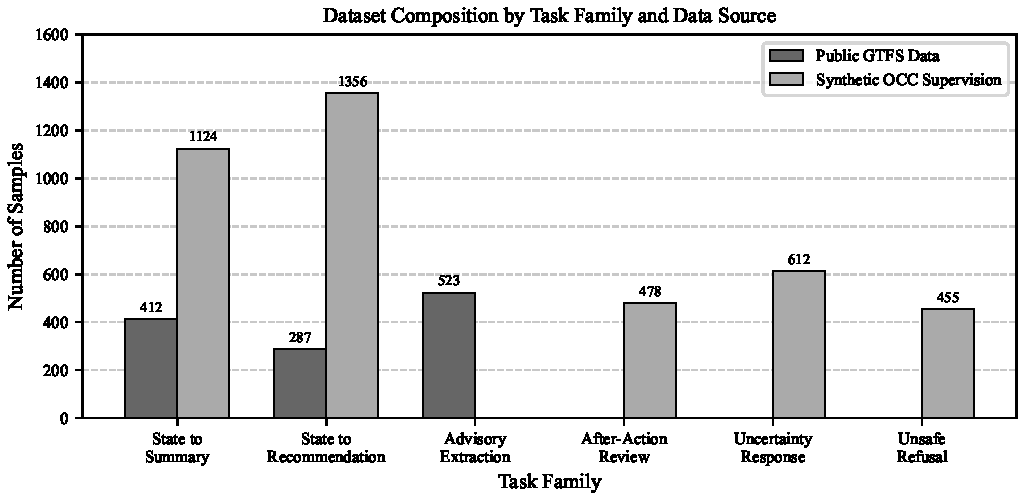
\includegraphics[width=0.95\textwidth]{figures/figure1_dataset_composition.pdf}
    \caption{Dataset composition by task family and data source. The benchmark spans six task families with contributions from public GTFS data, synthetic OCC supervision, and constructed operational procedures. State-to-summary and state-to-recommendation tasks comprise the largest portions, reflecting the primary OCC decision support focus.}
    \label{fig:composition}
\end{figure*}

\begin{figure*}[t]
    \centering
    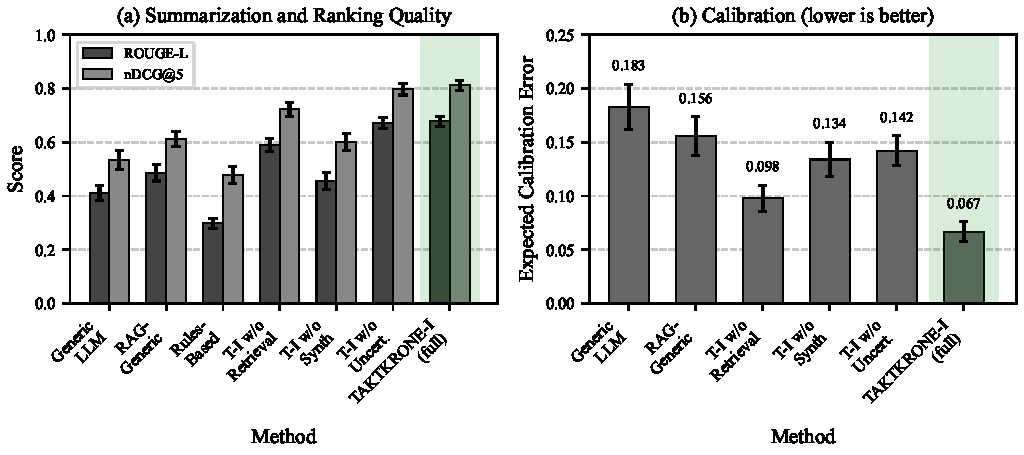
\includegraphics[width=0.95\textwidth]{figures/figure2_benchmark_results.pdf}
    \caption{Benchmark performance comparison across methods with 95\% confidence intervals. TAKTKRONE-I outperforms generic LLM and RAG baselines across summarization (ROUGE-L), recommendation ranking (nDCG@5), and calibration (ECE, lower is better). Ablations demonstrate the importance of retrieval grounding and synthetic OCC supervision.}
    \label{fig:results}
\end{figure*}

\begin{figure*}[t]
    \centering
    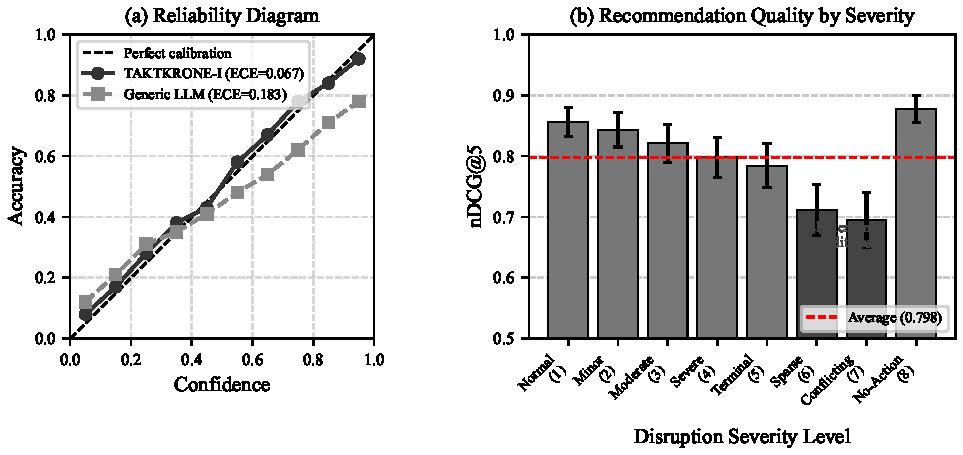
\includegraphics[width=0.95\textwidth]{figures/figure3_calibration_operational_effect.pdf}
    \caption{Calibration analysis and operational effect. Left: Reliability diagram comparing TAKTKRONE-I (ECE=0.067) against the generic LLM baseline (ECE=0.183), showing improved alignment between stated confidence and empirical accuracy. Right: Recommendation quality (nDCG@5) by disruption severity level, demonstrating stable performance across normal operations through severe disruptions with modest degradation under sparse telemetry conditions.}
    \label{fig:calibration}
\end{figure*}

\end{document}
